% SPDX-FileCopyrightText: Copyright (c) 2020-2025 Yegor Bugayenko
% SPDX-License-Identifier: MIT

\documentclass[12pt,twoside]{book}
\usepackage{../iccq}

\newwrite\pages
\immediate\openout\pages=\jobname.pages

\begin{document}

\blankleaf

\thispagestyle{empty}
\begin{center}
Proceedings

\vspace{1in}

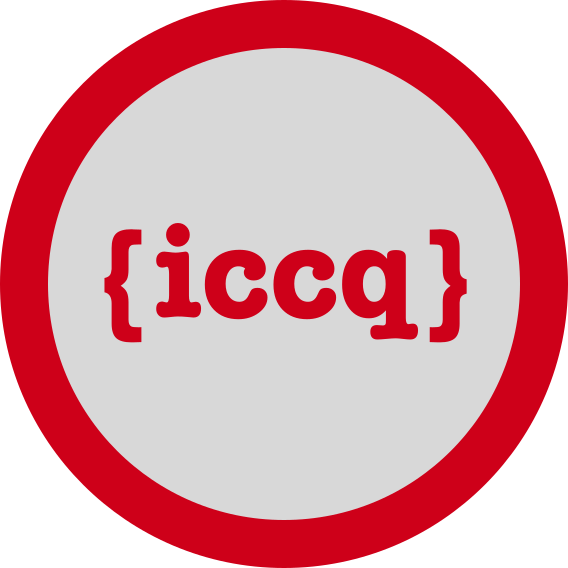
\includegraphics[height=1in]{../../logo}

\vspace{0.5in}

{\Large International Conference on Code Quality\\[12pt]
ICCQ 2021}

\vspace{0.5in}

Moscow, Russia\\
27 March 2021

\vspace{3in}

\begin{multicols}{3}
\includegraphics[height=0.8in]{../images/ieee-cs-logo}
\columnbreak

Los Alamitos, California\\
Washington $\bullet$ Tokyo

\columnbreak
\includegraphics[height=0.8in]{../images/ieee-cps-logo}
\end{multicols}
\end{center}


\iccqTOC

\clearpage
\thispagestyle{empty}
\addcontentsline{toc}{section}{Copyright}

{\small
\begin{center}
Copyright \copyright{} \the\year{}
by The Institute of Electrical and Electronics Engineers, Inc.\\
All rights reserved.
\end{center}

Copyright and Reprint Permissions: Abstracting is permitted with credit to the source. Libraries may photocopy beyond the limits of US copyright law, for private use of patrons, those articles in this volume that carry a code at the bottom of the first page, provided that the per-copy fee indicated in the code is paid through the Copyright Clearance Center,
\nospell{222 Rosewood Drive, Danvers, MA 01923}.

Other copying, reprint, or republication requests should be addressed to: IEEE Copyrights Manager, IEEE Service Center,
\nospell{445 Hoes Lane, P.O. Box 133, Piscataway, NJ 08855-1331}.

The papers in this book comprise the proceedings of the meeting mentioned on the cover and title page. They reflect the authors’ opinions and, in the interests of timely dissemination, are published as presented and without change. Their inclusion in this publication does not necessarily constitute endorsement by the editors, the IEEE Computer Society, or the Institute of Electrical and Electronics Engineers, Inc.

\begin{center}
ISBN-13: \input{isbn.txt} \\
Part No.: \input{part.txt}
\end{center}

\begin{center}
Additional copies may be ordered from:
\end{center}

\nospell{\begin{center}\scriptsize
\begin{multicols}{3}
IEEE Computer Society\\
Customer Service Center\\
10662 Los Vaqueros Circle\\
P.O. Box 3014\\
Los Alamitos, CA 90720-1314\\
Tel: + 1 800 272 6657\\
Fax: + 1 714 821 4641\\
http://computer.org/cps\\
cps@computer.org

\columnbreak

IEEE Service Center\\
445 Hoes Lane\\
P.O. Box 1331\\
Piscataway, NJ 08855-1331\\
Tel: + 1 732 981 0060\\
Fax: + 1 732 981 9667\\
http://shop.ieee.org/store/\\
customer-service@ieee.org

\columnbreak

IEEE Computer Society\\
Asia/Pacific Office\\
Watanabe Bldg., 1-4-2\\
Minami-Aoyama\\
Minato-ku, Tokyo 107-0062\\
JAPAN\\
Tel: + 81 3 3408 3118\\
Fax: + 81 3 3408 3553\\
tokyo.ofc@computer.org
\end{multicols}
\end{center}

\begin{center}
Editorial production by \nospell{Cristina Ceballos}\\
Cover art production by \nospell{Hector Torres}
\end{center}

% \begin{center}
% \includegraphics[height=0.5in]{../images/ieee-cs-logo}
% \quad\quad
% \includegraphics[height=0.5in]{../images/ieee-cps-logo}
% \end{center}

\begin{center}
IEEE Computer Society\\
Conference Publishing Services (CPS)\\
http://www.computer.org/cps
\end{center}

}

\begin{center}
\begin{multicols}{3}
\includegraphics[height=0.4in]{../images/ieee-cs-logo}
\columnbreak

{\small \nospell{Los Alamitos}, California\\
Washington $\bullet$ Tokyo}

\columnbreak
\includegraphics[height=0.4in]{../images/ieee-cps-logo}
\end{multicols}
\end{center}


\intro{parts/preface-program}

\intro{parts/preface-org}

\cleardoublepage
\sect{Organization}

\newcommand\pc[2]{\item #1 \\* {\small\color{gray} #2}}

\begin{multicols}{2}
\raggedright
Steering Committee

\begin{itemize}
\pc{\nospell{Hou Rui}}{\nospell{Director of Huawei MRC}}
\pc{\nospell{Alexander Tormasov}}{\nospell{Rector of Innopolis University}}
\end{itemize}

Program Committee

\begin{itemize}
\pc{\nospell{Karim Ali}}{\nospell{University of Alberta}}
\pc{\nospell{Luciano Baresi}}{\nospell{Politecnico di Milano}}
\pc{\nospell{Carl Friedrich Bolz-Tereick}}{\nospell{Heinrich-Heine-Universität Düsseldorf}}
\pc{\nospell{William J. Bowman}}{\nospell{University of British Columbia}}
\pc{\nospell{Laura M. Castro}}{\nospell{Universidade da Coruña}}
\pc{\nospell{Shigeru Chiba}}{\nospell{University of Tokyo}}
\pc{\nospell{Christian Hammer}}{\nospell{University of Passau}}
\pc{\nospell{Mats Heimdahl}}{\nospell{University of Minnesota}}
\pc{\nospell{Robert Hirschfeld}}{\nospell{University of Potsdam}}
\pc{\nospell{Alexandra Jimborean}}{\nospell{Uppsala University}}
\pc{\nospell{David H. Lorenz}}{\nospell{Open University of Israel}}
\pc{\nospell{Hidehiko Masuhara}}{\nospell{Tokyo Institute of Technology}}
\pc{\nospell{Hausi A. Müller}}{\nospell{University of Victoria}}
\pc{\nospell{Yongjun Park}}{\nospell{Hanyang University}}
\pc{\nospell{Gennady Pekhimenko}}{\nospell{University of Toronto}}
\pc{\nospell{Veselin Raychev}}{\nospell{ETH}}
\pc{\nospell{Tiark  Rompf}}{\nospell{Purdue University}}
\pc{\nospell{Yulei Sui}}{\nospell{University of Technology Sydney}}
\pc{\nospell{Will Tracz}}{\nospell{IFIP}}
\pc{\nospell{Laurie Williams}}{\nospell{North Carolina State University}}
\pc{\nospell{Tuba Yavuz}}{\nospell{University of Florida}}
\end{itemize}

Organizers

\begin{itemize}
\item \nospell{Yegor Bugayenko} (Chair)
\item \nospell{Sergey Belov}
\item \nospell{Andrey Kuleshov}
\item \nospell{Sergei Prokhorov}
\end{itemize}
\end{multicols}


% SPDX-FileCopyrightText: Copyright (c) 2020-2025 Yegor Bugayenko
% SPDX-License-Identifier: MIT

\cleardoublepage
\sect{Sponsors and Partners}

\newcommand\partner[3]{\includesvg[#1]{../../images/#2.svg} \\ #3}

\partner{height=0.7in}{partners/iu}{Innopolis University}

\partner{height=0.7in}{partners/spbu}{St. Petersburg State University}

\partner{height=0.8in}{partners/hse}{Higher School of Economics}


\fancypagestyle{ieee}{\fancyfoot[C]{
  \head{\paging} \\
  \head{\input{isbn.txt}\unskip/21/\$31.00 \textcopyright{} \the\year{} IEEE}
}}

\newcounter{start}

\blankleaf
\index{Wang, Quanyu}
\index{Liutova, Daria}
\index{Malykh, Valentin}
\paper{29}
  {\nospell{Multilingual Code Comment Translation: A Case Study on Chinese, English, and Russian}}
  {\nospell{Quanyu Wang, Daria Liutova, and Valentin Malykh}}

\blankleaf
\index{Menshutin, Aleksei}
\paper{34}
  {\nospell{Path-Minimal Objects in ArkTS Symbolic Execution}}
  {\nospell{Aleksei Menshutin}}

\blankleaf
\index{Baranov, Alexander}
\index{Eroschenko, Artem}
\index{Vesyoly, Denis}
\index{Voronchuk, Ilya}
\paper{36}
  {\nospell{Modeling and Software Development the Virtual Lab \enquote{Tonomura's single-electron double slit experiment}}}
  {\nospell{Alexander V. Baranov, Artem A. Eroschenko, Denis A. Vesyoly, and Ilya I. Voronchuk}}

\blankleaf
\index{Dikov, Alexander}
\index{Zvorygin, Vladimir}
\index{Malykh, Valentin}
\paper{39}
  {\nospell{Diffusion vs Autoregression: An Empirical Study on Code Comment Translation}}
  {\nospell{Alexander Dikov, Vladimir Zvorygin, and Valentin Malykh}}

\blankleaf
\iccqIndex

\end{document}
